%\documentclass[12pt,a4paper]{report}
\documentclass[12pt,a4paper]{article}

\usepackage[brazil]{babel}
\usepackage[utf8]{inputenc}
\usepackage[T1]{fontenc}
\usepackage{graphicx,url}
\usepackage{hyperref}
%\usepackage{mathptmx}
\usepackage{lipsum}
\usepackage{booktabs}
\usepackage{pifont}
\usepackage{textcomp}
\usepackage{amsmath,amssymb}
\usepackage{listings}
\usepackage[scaled=0.8]{beramono}
\usepackage{xspace}
\usepackage{pdfpages}
\usepackage{listings}
\usepackage{xcolor}

\pdfgentounicode=1

\newcommand{\HRule}{\rule{\linewidth}{0.5mm}}

\lstdefinestyle{c}{%
    language=C,
    basicstyle=\ttfamily,
    numbers=left,
    breaklines=true,
    belowcaptionskip=1\baselineskip,
    aboveskip=1\baselineskip,
    belowskip=1\baselineskip,
    moredelim=**[is][\color{red}]{@}{@}
}

\lstset{%
    basicstyle=\ttfamily,
    aboveskip=1\baselineskip,
    belowskip=1\baselineskip,
    extendedchars=true,
    literate={á}{{\'a}}1 {ã}{{\~a}}1 {é}{{\'e}}1
}

\renewcommand{\lstlistingname}{Código}

\begin{document}

\begin{titlepage}

\begin{center}


\includegraphics[width=1.0\textwidth]{img/unb_logo.jpg}~\\[1cm]

\textsc{\Large Programação Paralela}\\[0.5cm]

% Title
\HRule\\[0.4cm]
{\huge \bfseries Relatório do Exercício 3\\[0.4cm]}
\HRule\\[1.5cm]

% Author and Supervisor
\begin{minipage}{0.4\textwidth}
\begin{flushleft} \large
\textit{Autor:}\\
\small{Alexandre Lucchesi Alencar}
\end{flushleft}
\end{minipage}
\begin{minipage}{0.4\textwidth}
\begin{flushright} \large
\textit{Professor:}\\
\small{George Luiz Medeiros Teodoro}
\end{flushright}
\end{minipage}

\vfill

% Bottom of the page
{\large \today}

\end{center}

\end{titlepage}



\section{Introdução}
Este relatório tem como objetivo apresentar os resultados obtidos a partir da
execução do terceiro exercício de programação paralela~\cite{exercise}, que
consiste na implementação de uma árvore de redução de soma (\textit{sum tree})
utilizando Message Passing Interface (MPI)~\footnote{Neste trabalho, utilizou-se
a implementação OpenMPI para Mac OS X, instalada a partir do utilitário
Homebrew.}. Primeiramente, os aspectos principais do algoritmo desenvolvidos são
apresentados. Em seguida, é realizada uma análise de desempenho comparando os
tempos de execução do algoritmo em diversas configurações, isto é, variando-se o
número de processos e a quantidade de números de ponto-flutuante a serem
somados. O código-fonte completo deste trabalho, incluindo os arquivos
\LaTeX\xspace que compõem este relatório, estão publicamente disponíveis no
GitHub~\footnote{\url{https://github.com/alexandrelucchesi/parallel-programming-ex03}}.

\subsection{\textit{Hardware} Utilizado}
\label{sec:hardware}

\begin{itemize}
    \item Processador: Intel Core i7
    \item Velocidade: 2 GHz
    \item Número de processadores: 1
    \item Número de \textit{cores} reais: 2
    \item Número de \textit{cores} virtuais: 4 (HyperThreading)
    \item L1 cache: 32KB
    \item L2 cache (per core): 256KB
    \item L3 cache: 4MB
\end{itemize}


\section{O Algoritmo}


\subsection{Artefatos Desenvolvidos}
O programa desenvolvido possui duas funcionalidades principais: (i) geração de
um arquivo de dados contendo um número arbitrário de valores de ponto-flutuante;
(ii) e processamento de um arquivo de dados retornando a soma dos elementos e o
tempo de execução do algoritmo. Além do programa principal, foram desenvolvidos
dois \textit{scripts bash}: um para facilitar a execução do programa principal,
encapsulando a chamada ao \texttt{mpiexec} (ou \texttt{mpirun}), e outro para
automatizar os testes da aplicação. Esses artefatos são descritos a seguir.

\begin{itemize}
    \item \texttt{main.c}: programa em C contendo o código-fonte da aplicação.
        Após compilado com o \texttt{mpicc} (vide Makefile), pode ser executado
        chamando-se o \textit{script} \texttt{run.sh} passando-se o número de
        processos e o arquivo de dados. O \texttt{run.sh} executará o programa
        usando o \texttt{mpiexec} e passando esses dois argumentos, que são
        recebidos via \texttt{scanf()}. A saída do programa é uma linha contendo
        dois números: o primeiro representa o resultado da soma dos números de
        ponto-flutuante e o segundo, o tempo de execução do algoritmo de redução
        em milisegundos (desconsiderando o tempo de entrada de dados).
% TODO: Update text below!
	\item \texttt{test.sh}: \textit{script} desenvolvido para automatizar os
		testes da aplicação. Recebe como entrada 4 argumentos, em ordem:
		\begin{itemize}
			\item \texttt{max\_threads}: número máximo de \textit{threads}. O
				\textit{script} varia o número de \textit{threads} de 1 até
				\texttt{max\_threads}.
            \item \texttt{max\_tosses}: ordem máxima do número de lançamentos,
                isto é, o \textit{script} executa a aplicação variando o número
                de lançamentos, começando em $10^2, 10^3$ até
                $10^{max\_tosses}$.
			\item \texttt{max\_runs}: número máximo de vezes em que o programa
				deve ser executado em uma mesma configuração.
			\item \texttt{max\_time}: \textit{timeout} de execução, ou seja, se o
				programa não encerrar a execução nesse tempo, ele é finalizado.
		\end{itemize}
\end{itemize}


\subsection{Geração do Arquivo de Dados}
\label{sec:data-gen}
Para a geração de quantidades configuráveis de números de ponto-flutante em um
formato apropriado para servir de entrada para o programa, pode-se executar o
binário proveniente do processo de compilação diretamente. Por exemplo, para
gerar um arquivo de dados, \texttt{numbers.dat}, contendo, por exemplo, 64
elementos, basta executar o binário passando-se a \textit{flag} \texttt{-gen},
conforme descrito a seguir:

\begin{lstlisting}[language=bash]
$ make      # Gera o binário com nome: 'sumtree'.
$ ./sumtree -gen numbers.dat 64
\end{lstlisting}

Uma outra opção disponível é a \texttt{-{}-help}, que exibe informações de uso da
aplicação.


\subsection{Função de ``Espalhamento''}
Para distribuir os dados entre os diferentes processos, foram criadas duas
funções:

\begin{lstlisting}[style=c, numbers=none]
void scather(int my_rank, int comm_sz,
    unsigned int *my_count, float **my_nums);
void scather_intercalate(int my_rank, int comm_sz,
    unsigned int *my_count, float **my_nums);
\end{lstlisting}

Uma sempre pode ser utilizada no lugar da outra sem alterar o resultado final
(note que a assinatura é a mesma). A única diferença está na política de
atribuição dos números aos processos. Internamente, o processo com
\texttt{my\_rank} igual a zero é sempre o responsável por ler o arquivo de dados
e dividir os números entre os \texttt{comm\_sz} processos, retornando em
\texttt{my\_count} e \texttt{my\_nums} a quantidade de elementos e os números,
respectivamente.

No caso da \texttt{scather}, a quantidade total de números (lida do arquivo de
entrada) é dividida pelo número de processos (\texttt{comm\_sz}) e o resultado
(\texttt{res}) obtido é utilizado para atribuir sequencialmente os números aos
processos, ou seja, o processo 0 recebe os números indexados pelo intervalo $[0,
res - 1]$, o processo 1 recebe $[res, 2 \times res - 1]$, e assim por diante.

Por outro lado, a \texttt{scather\_intercalate} intercala os números entre os
processos, varrendo o vetor e atribuindo o elemento no índice $i$ ao processo $i
\bmod comm\_sz$. 


\subsection{Evitando \textit{Deadlocks}}
Na implementação do MPI utilizada, ambas as primitivas \texttt{Send()} e
\texttt{Recv()} são ``blocantes''. Isso significa que cuidado adicional deve ser
tomado para que não ocorram \textit{deadlocks}. O trecho de
código~\ref{code:deadlock} apresenta como a função \texttt{reduce\_sumtree()}
foi projetada para evitar a ocorrência de \textit{deadlocks}.

\begin{minipage}{\linewidth}
\begin{lstlisting}[frame=single, style=c, label={code:deadlock},
    caption={Ordem das primitivas MPI\_Send() e MPI\_Recv() na função \texttt{reduce\_sumtree()}.}]
...
if (my_rank % 2 == 0) {
    int dst = my_rank + 1;

    /* Send first half (or the last) of `nums[]` to `dst`. */
    for (unsigned int i = 0; i < half_or_one; i++)
        @MPI_Send(nums + i, 1, MPI_FLOAT, dst, 2, MPI_COMM_WORLD);@

    /* Receives half (or the last) of `dst`'s `nums[]` and accumulates into `*sum`. */
    for (unsigned int i = 0; i < half_or_one; i++) {
        @MPI_Recv(&his_num, 1, MPI_FLOAT, dst, 2, MPI_COMM_WORLD,@
            @MPI_STATUS_IGNORE);@
        (*sum) += his_num;
    }
} else {
    int dst = my_rank - 1;

    /* Receives half (or the last) of `dst`'s `nums[]` and accumulates into `*sum`. */
    for (unsigned int i = 0; i < half_or_one; i++) {
        @MPI_Recv(&his_num, 1, MPI_FLOAT, dst, 2, MPI_COMM_WORLD,@
            @MPI_STATUS_IGNORE);@
        (*sum) += his_num;
    }

    /* Send first half (or the last) of `nums[]` to `dst`. */
    for (unsigned int i = 0; i < half_or_one; i++)
        @MPI_Send(nums + i, 1, MPI_FLOAT, dst, 2, MPI_COMM_WORLD);@
}
...
\end{lstlisting}
\end{minipage}

Se as primitivas \texttt{MPI\_Recv()} e \texttt{MPI\_Send()} aparecerem na mesma
ordem no \texttt{if} e no \texttt{else}, os processos entrarão em
\textit{deadlock}. Ao colocá-los de forma alternada, garante-se que para cada
\texttt{MPI\_Send()} existirá um \texttt{MPI\_Recv()} e vice-versa.


\section{Resultados}
\label{sec:resultados}
Executou-se o \textit{script} de testes (\texttt{test.sh}) passando-se como
argumentos: 6 \textit{threads}, $10^{12}$ lançamentos, 5 execuções por
configuração e \textit{timeout} de 24 minutos. Além disso, utilizou-se o
utilitário de linha de comando \texttt{time} para calcular o tempo total de
execução dos testes. O resultado é apresentado a seguir.

\begin{verbatim}
$ time sh test.sh 6 12 5 1440

real    633m8.800s
user    1503m45.812s
sys     1m9.481s
\end{verbatim}

O valor \texttt{real} é o tempo real (``relógio de parede'') transcorrido desde
o início da execução do programa até seu término (incluindo períodos de
bloqueio, etc). Por outro lado, os valores de \texttt{user} e \texttt{sys} se
referem ao tempo de CPU usado pelo processo em modo usuário e modo
\textit{kernel}, respectivamente. Dessa forma, a execução dos testes
responsáveis por gerar as tabelas de \textit{benchmark} levou quase 11 horas
para ser concluída.

O \textit{script} \texttt{test.sh} gera como saída $2 \times max\_threads$
arquivos no formato CSV\@ (no exemplo acima, 12 arquivos). Cada tabela é
indexada pelo número de lançamentos (no exemplo acima, de $10^2$ à $10^{12}$) e
o número da execução (no exemplo acima, de 1 a 5).  Metade possui o prefixo
\texttt{pi\_{n}}, onde \texttt{n} é o número de \textit{threads} utilizado,
representando os valores aproximados de pi calculados. A outra metade possui
prefixo \texttt{time\_{n}}, e contém os valores dos tempos de execução. O valor
\texttt{*} representa um \textit{timeout}. Em poucas palavras, tem-se 2 arquivos
por quantidade de \textit{threads} contendo as duas saídas do programa: o valor
estimado de pi e o tempo de execução do algoritmo.

As tabelas a seguir apresentam os resultados dos testes. Observa-se que para uma
quantidade de lançamentos pequena ($10^2$ e $10^3$), o tempo de execução do
algoritmo sequencial é melhor do que nas demais configurações. Isto ocorre
porque os ganhos obtidos da paralelização do algoritmo não são suficientes para
cobrir o custo de se criar as \textit{threads}. Ao aumentar o número
de lançamentos para $10^4$, observa-se que o desempenho do algoritmo sequencial
já perde para algumas configurações, sendo inferior ao obtido com 3 e 4
\textit{threads}. A partir de $10^5$ lançamentos, o desempenho do algoritmo
sequencial se torna inferior a todas as demais configurações.

É importante notar que para o algoritmo sequencial e para as configurações 2 e 3
\textit{threads}, o programa excedeu o tempo máximo de execução pré-estabelecido
(24 minutos). No entanto, para as configurações 4, 5 e 6 \textit{threads}, esse
tempo não foi atingido, evidenciando que o algoritmo paralelizado é escalável.
Além disso, observando-se os tempos de execução quando o número de lançamentos é
alto ($10^{10}$ e $10^{11}$), conclui-se que o maior desempenho é alcançado
utilizando-se 4 \textit{threads}. Isso está relacionado com o fato de que o
processador utilizado possui 2 \textit{cores} em
HyperThreading~\ref{sec:hardware}.

Em linhas gerais, para $10^{6}$ lançamentos e 4 \textit{threads}, foi possível
obter o \textit{speedup} máximo: $\approx 252\%$. Em contrapartida, para
$10^{2}$ lançamentos e 6 \textit{threads}, ocorreu o pior \textit{speedup}:
$\approx 4.5\%$. Esse resultado era esperado, uma vez que o custo de se
gerenciar 6 \textit{threads} para calcular apenas 100 números é muito alto.

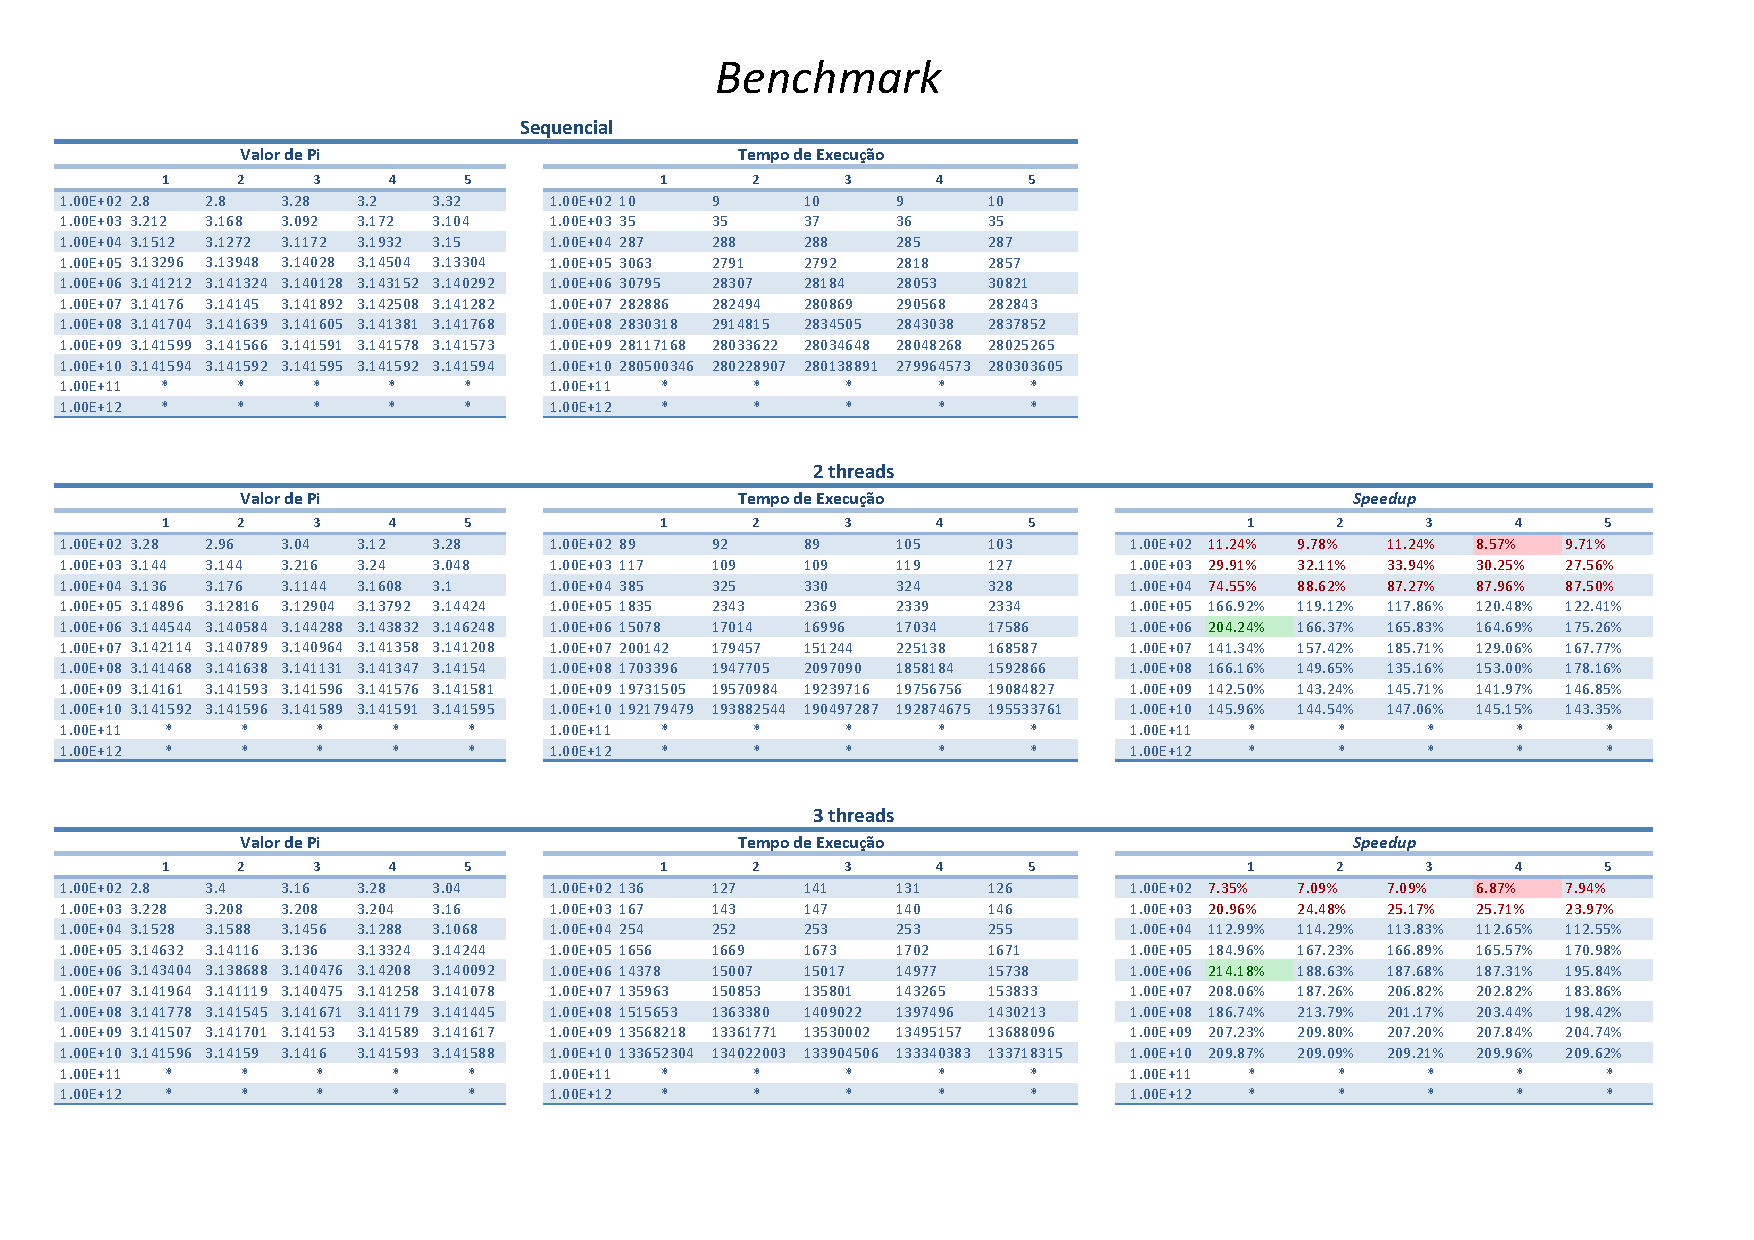
\includepdf[pages={1-},scale=1.0,landscape=true]{bench.pdf}

\section{Conclusão}
Este trabalho possibilitou uma maior compreensão acerca de modelos de
programação baseados em trocas de mensagem, em particular, que utilizam
primitivas \texttt{Send()} e \texttt{Recv()}, através da implementação de uma
árvore de redução de soma usando MPI\@.

O algoritmo desenvolvido possibilita a simulação de reduções usando um número
grande de processos, utilizando as primitivas citadas anteriormente para
realizar somas intermediárias até chegar na redução a partir de uma \emph{Sum
Tree}. Uma análise dos tempos de execução do algoritmo evidenciou ganhos de
desempenho (\textit{speedup}) de até 252\% em relação à versão sequencial.

Por fim, é válido ressaltar que o o \textit{design} da aplicação (incluindo o
\textit{script} \texttt{test.sh}) permite variar de forma fácil as condições de
teste, permitindo a reprodução dos experimentos apresentados neste trabalho e
facilitando a experimentação com novas configurações. 

\bibliographystyle{plain}
\bibliography{references.bib}

\end{document}








